%% We use `subfiles' package
\documentclass[preamble.tex]{subfiles}
\begin{document}


\clearpage

\chapter{Results}
\label{ch:results}


\section{QuickHull}
\label{sec:QuickHull}

Throughout this chapter we will use a \name{Data Parallel Haskell} implementation of the QuickHull algorithm that computes the convex hull of a finite set of points in the plane. It derives its name from the QuickSort algorithm and similarly uses a divide and conquer approach.

The convex hull for a set of points in the plane can be visualised as a polygon formed by a rubber band stretched around the points. The smallest set of points forming the polygon that encloses all other points is called the convex hull.

The result of finding convex hull of a set of points can be seen on the right of Figure~\ref{fig:qh-result}. The same figure depicts the three steps of the sample run of QuickHull algorithm.


\subsection{QuickHull in \DPH}

The \DPH implementation of QuickHull closely follows the recursive solution:
\begin{enumerate}
  \item Finds the points with smallest and largest $x$ coordinates (lines 12 and 13 and Figure~\ref{fig:qh-result} left). These points are bound to be in the convex hull.

  \item The line between the two points forms two subsets of points, which will be processed recursively (line 8) by @QuickHullR@ function.

  \item The recursive @QuickHullR@ function, given a subset of points and a line, determines the point, on one side of the line, @far@thest from it (line 27). This point is also in the convex hull.

  \item @QuickHullR@ also filters out all points on the other side of the line (line 25), keeping only the points @above@ the line.

  \item The two ends of the line each form a new line with the @far@ point to be recursively processed (line 19).

  \item The previous three steps are repeated expanding the convex hull until no more points are left above any of the lines. The recursion has finished and the points forming the lines constitute the convex hull.
\end{enumerate}


\begin{figure}
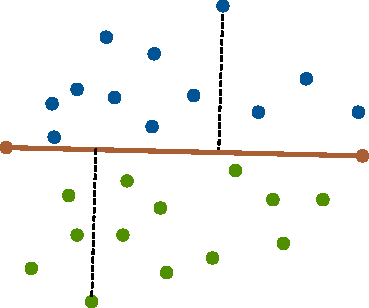
\includegraphics[width=0.3\textwidth]{img/Example-QuickHull-step1}~~~~~%
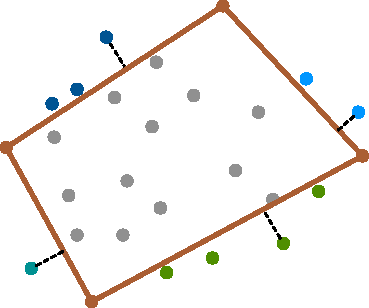
\includegraphics[width=0.3\textwidth]{img/Example-QuickHull-step2}~~~~~%
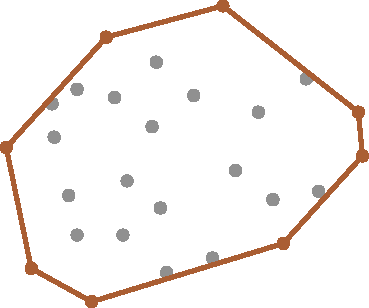
\includegraphics[width=0.3\textwidth]{img/Example-QuickHull-step3}%
\caption{Three steps of a sample run of data parallel QuickHull algorithm.}
\label{fig:qh-result}
\end{figure}


\begin{hscode}[%
  caption={\label{fig:dph-qh}\name{Data Parallel Haskell} implementation of QuickHull.},
  numbers=left,
]
type Point = (Double, Double)
type Line  = (Point,  Point)

quickHull :: [:Point:] -> [:Point:]
quickHull points
  | lengthP points == 0 = points
  | otherwise
  = concatP [: quickHullR points ends
                 | ends <- [: (minx, maxx), (maxx, minx) :] :]
  where
    xs   = [: x | (x, y) <- points :]
    minx = points !: minIndexP xs
    maxx = points !: maxIndexP xs

quickHullR :: [:Point:] -> Line -> [:Point:]
quickHullR points line@(start, end)
  | lengthP above == 0 = [:start:]
  | otherwise
  = concatP [: quickHullR above ends
                 | ends <- [:(start, far), (far, end):] :]
  where
    -- Find relative distance from each point to the line
    distances = [: distance p line | p <- points :]
    -- Only keep points above the line
    above = [: p | (p,c) <- zipP points distances, c > 0.0 :]
    -- Find the point farthest from the line
    far = points !: maxIndexP distances

-- Cross product used as distance-like measure
distance :: Point -> Line -> Double
distance (xo, yo) ((x1, y1), (x2, y2))
  = (x1 - xo) * (y2 - yo) - (y1 - yo) * (x2 - xo)
\end{hscode}



\subsection{QuickHull vectorisation}

The QuickHull program presented is a typical example of a divide and conquer algorithm. Recursive calls of @quickHullR@ function in most languages would be processed sequentially one at a time. However, in \DPH, the function is vectorised as described in Section~\ref{sec:Vectorisation} to give @quickHullR^@ of the following type:


\begin{hscode}[literate={^}{{$^\uparrow$}}1,]
-- Original
quickHullR  :: [:Point:] -> Line -> [:Point:]
-- Vectorised
quickHullR^ :: [:[:Point:]:] -> [:Line:] -> [:[:Point:]:]
\end{hscode}


The vectorised function is able to process not one, but an array of lines at a time. This means that the ``expansion'' of convex hull in every direction happens in one call of @quickHullR^@. In fact the three steps of vectorised QuickHull depicted in Figure~\ref{fig:qh-result} faithfully represent the only three calls to @quickHullR^@ required to find the convex hull.



\subsection{QuickHull in the backend}

The vectorised @quickHullR^@ function takes a \*nested parallel array* of points @[:[:Point:]:]@ as its first argument. It was discussed in Section~\ref{sec:Flattening}, that such nested arrays are represented using \*segmented* arrays in the backend.

Recalling that an \*array of pairs* is repesented as a \*pair of arrays* (Section~\ref{sec:DPH-Data-Representation}), the \*Flattening transform* represents a \*nested array* of @Point@ as two data arrays and a segment descriptor:


% For drawing rules of width of multiples of fixed char width
% E.g. \seg{4} will give ----
\newlength\fixedcharwidth
\settowidth{\fixedcharwidth}{\code{a}}
\newcommand\seg[1]{\rule{#1\fixedcharwidth}{1pt}}

% xs:   [: [:3:], [:4, 2, 2, 4:], [:8, 7, 7,  9:], [:9, 10, 8:], [:4:] :]
% ys:   [: [:3:], [:7, 8, 9, 9:], [:8, 7, 9, 10:], [:5,  3, 1:], [:0:] :]

\begin{hscode}
type Point = (Double, Double)

Points:
  [:
     [:(3,3):],
     [:(4,7), (2,8),  (2,9), (4,9):],
     [:(8,8), (7,7),  (7,9), (9,10):],
     [:(9,5), (10,3), (8,1):],
     [:(4,0):]
  :]

                        %$\Downarrow$%

segd: [ 1, 4, 4, 3, 1 ]
        %\seg{1}~~\seg{10}~~\seg{11}~~\seg{8}~~\seg{1}%
xs:   [ 3, 4, 2, 2, 4, 8, 7, 7,  9, 9, 10, 8, 4 ]
ys:   [ 3, 7, 8, 9, 9, 8, 7, 9, 10, 5,  3, 1, 0 ]
\end{hscode}


While the the second argument to the function is a \*flat* array of @Line@, it too is represented as four separate arrays in accordance to the type of @Line@. For example:


\begin{hscode}
type Line = (Point, Point)

x1s = [2, 1, 4, 8, 9]
y1s = [1, 5,10, 6, 0]
x2s = [1, 4, 8, 9, 2]
y2s = [5,10, 6, 0, 1]
\end{hscode}


Overall, the time @quckHullR^@ function goes through the following transformations before it is compiled using the backend library of collective array operations (such as \LiveFusion)\footnote{I omit certain internal wrapper types to simplify the example.}:

\begin{hscode}[literate={^}{{$^\uparrow$}}1,]
quickHullR  :: [:Point:] -> Line -> [:Point:]

                        %$\Downarrow$%   Lifting transform

quickHullR^ :: [:[:Point:]:] -> [:Line:] -> [:[:Point:]:]

                        %$\Downarrow$%   Flattening transform

quickHullR_ :: Array Int                      -- segment descriptor
            -> Array Double -> Array Double   -- points
            -> Array Double -> Array Double   -- line starts
            -> Array Double -> Array Double   -- line ends            
            -> Array Double -> Array Double   -- convex hull points
\end{hscode}



\subsection{The heart of QuickHull: Segmented FilterMax}
\label{sec:FilterMax}

By the time a \DPH program is compiled in the backend, it is composed of a large data flow graph of flat and segmented array combinators.

For example the complete data flow diagram for QuickHull is shown on Figure~\ref{fig:DFD-QuickHull}.


\begin{figure}
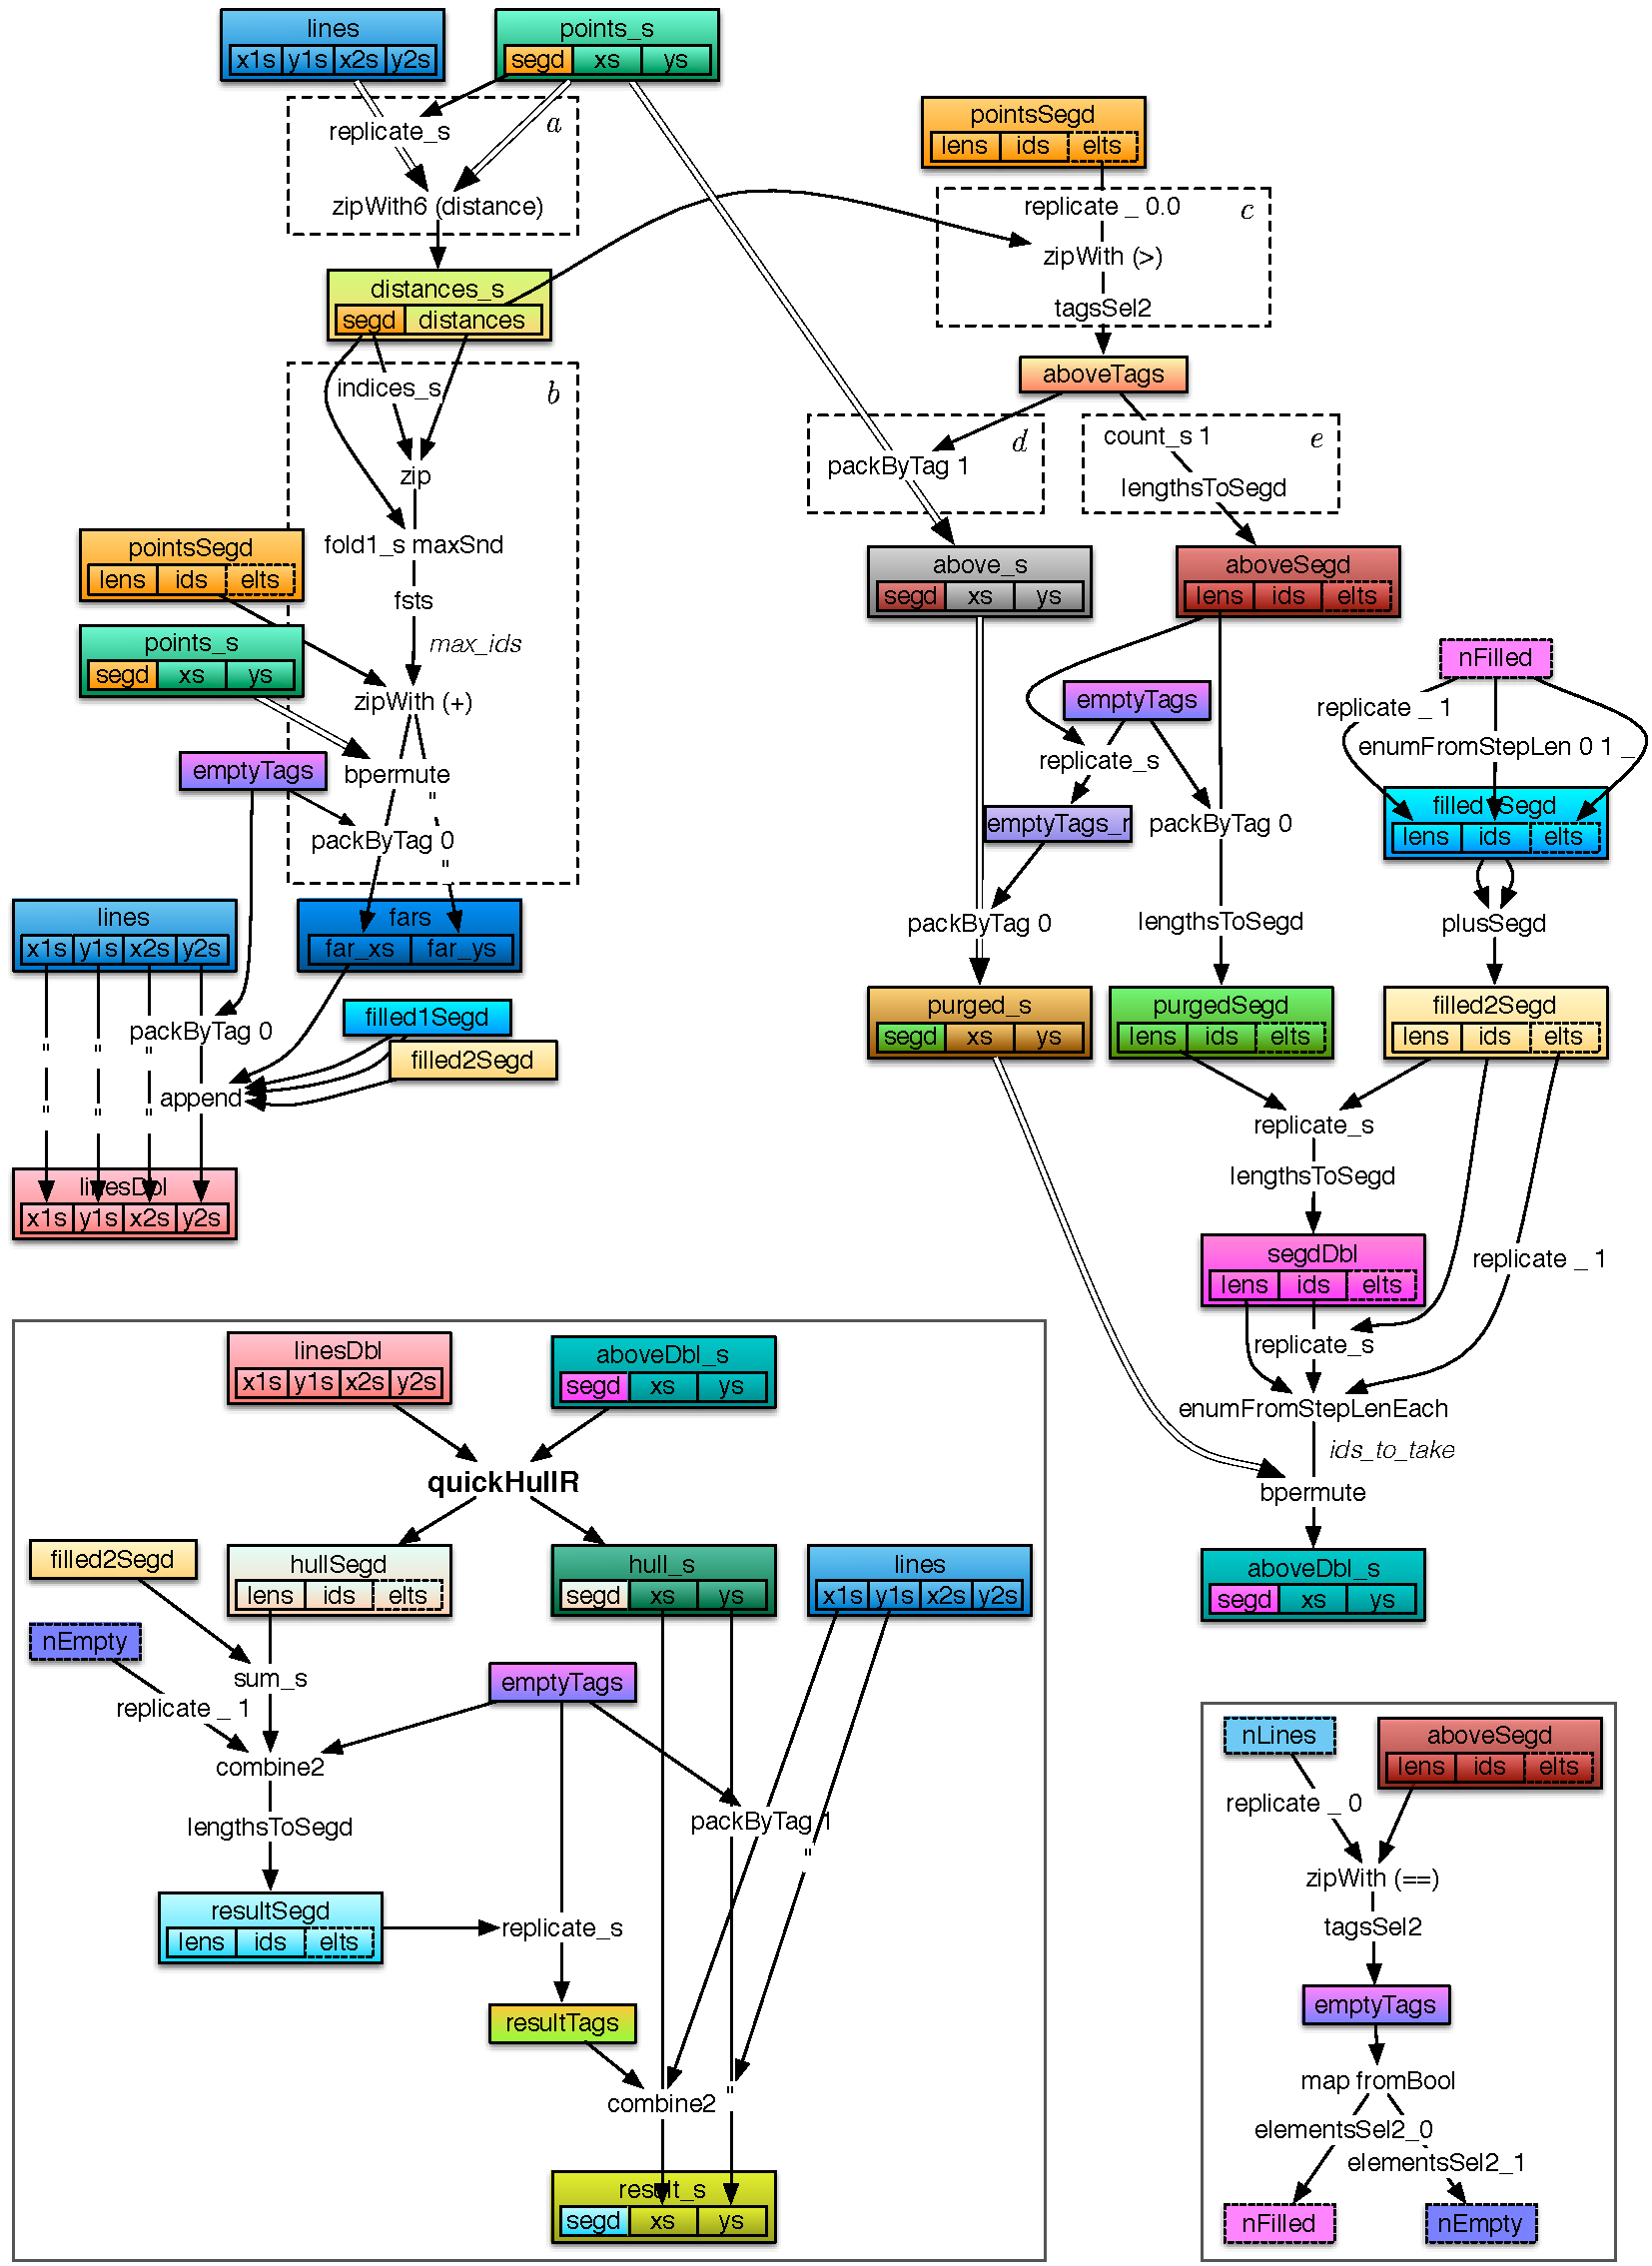
\includegraphics[width=1.1\textwidth, center]{img/DFD-QuickHull}
\caption{Data flow diagram of array combinators generated by the vectoriser for \code{quickHullR} function.}
\label{fig:DFD-QuickHull}
\end{figure}


While the graph consists of over 40 array combinators, roughly $^2/_3$ of its runtime the QuickHull program spends in what we will refer to as \name{segmented FilterMax}. With reference to the data flow diagram, in each recursive step of QuickHull it uses relative distances computed by group of combinators \*a* to finds points above a number of lines (\*c*, \*d* and \*e*) as well as points farthest from each line (\*b*).

The complete implementation of \name{segmented FilterMax} using \LiveFusion interface is given in Appendix~\ref{sec:FilterMax-implementation}. It closely follows the implementation of QuickHull, done by the author by studying the \name{GHC Core} code generated by \DPH vectoriser\footnote{The complete hand-vectorised implementation of QuickHull is available at \url{http://github.com/ghc/packages-dph/tree/master/dph-examples/examples/spectral/QuickHull/handvec}}.



\subsection{\StreamFusion and \FilterMax}

In the previous section we have identified groups of combinators \*a* to \*e* that make up the functionality of segmented \FilterMax. The grouping is not incidental. When vectorised \QuickHull is compiled using the \StreamFusion framework the combinators in each of these groups get fused together.

However, the fusion stops at the boundaries of each of these groups.

The \FilterMax example exhibits both problems with \StreamFusion identified in Section~\ref{sec:problems}: the inability to fuse producers with multiple consumers and the duplicated counters.


\subsubsection{Multiple consumers}

Both the filtering part of \FilterMax, finding points above the lines (\*c*, \*d*, \*e*) and the part finding the farthest points (\*b*) rely on the distances to be computed first (\*a*). Because of inherent limitation of fusion systems based on rewrite rules covered in Section~\ref{sec:multiple-consumers}, \StreamFusion is unable to fuse the producer of the segmented @distances_s@ array into the two consumers albeit they could easily be computed in the same loop.

For the same reason combinator groups \*d* and \*e* cannot be fused with group \*c* that produces an array of boolean tags specifying which points should be kept and which filtered out.

\LiveFusion on the other hand is able to fuse all combinator groubs \*a* through \*e* into a single (nested) loop.


\subsubsection{Duplicated loop counters}

With arrays of points being represented by two arrays and arrays of lines -- by four arrays, any computation involving their point-wise processing adds a separate counter variable and bounds check in \StreamFusion. This problem has been discussed in Section~\ref{sec:duplicated-counters} and solved in \LiveFusion using rates (Section~\ref{sec:rates}).

Referring to the \FilterMax example, @zipWith6@ combinator from group \*a* uses 6 separate counters for each of the input arrays and one for the output. Similarly, @zip@ and @zipWith@ combinators of groups \*b* and \*c* use 3 counters each.



\subsection{Evaluation}

The benchmarking in this section has been carried out using an implementation of \QuickHull vectorised by hand replicating the intermediate \name{GHC Core} code produced by \DPH vectoriser. It is expressed using array combinators that can be compiled either using a \StreamFusion or a \LiveFusion based backend library.

A variant of \QuickHull that uses \LiveFusion to compute \FilterMax has been compiled. As of this writing \LiveFusion is able to dynamically generate and load fused code. However, it does not cache the compiled code. To avoid recompiling the same combinator graph in each recursive step of \QuickHull, the pre-generated code of \FilterMax has been compiled in. Additional compilation costs are factored into the results where appropriate.

Both programs have been run on 10, 20, 25, 40 and 50 million points.
Figure~\ref{fig:Eval-QuickHull} shows the runtime of the complete \QuickHull program. In one instance it uses \StreamFusion throughout. In another it substitutes \LiveFusion generated code to compute \FilterMax.

\ref{fig:Eval-QuickHull-numbers}


\begin{figure}
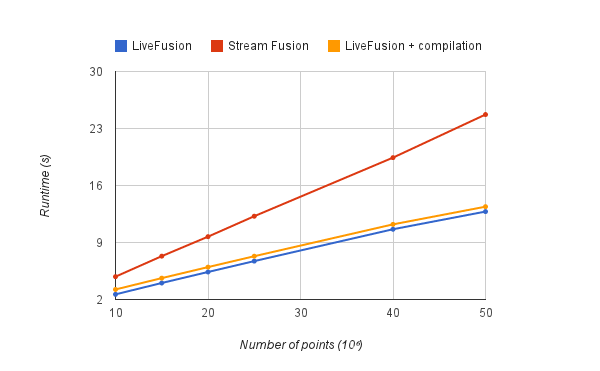
\includegraphics[center]{img/Eval-QuickHull}
\caption{Runtime of vectorised QuickHull with \FilterMax fused by \StreamFusion and \LiveFusion.}
\label{fig:Eval-QuickHull}
\end{figure}


\begin{figure}
\csvautotabular{Results-QuickHull.csv}
\caption{Runtime of vectorised QuickHull with \FilterMax fused by \StreamFusion and \LiveFusion (measured in milliseconds).}
\label{fig:Eval-QuickHull-numbers}
\end{figure}


However, given the divide-and-conquer nature of \QuickHull and the decreasing number of points at every step

\begin{figure}
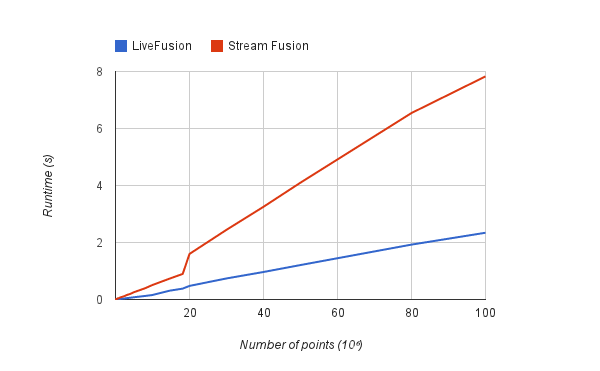
\includegraphics[center]{img/Eval-FarAndAboves}
\end{figure}

\begin{figure}
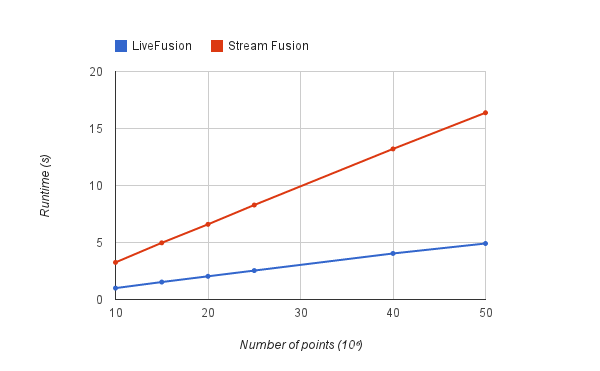
\includegraphics[center]{img/Eval-FarAndAboves-Overall}
\end{figure}

\clearpage
\section{Compilation time and amortisation}


\IfNotCompilingAll{\bibliography{bib}}

\end{document}